\documentclass[conference]{IEEEtran}
\usepackage[top=0.75in, bottom=1.0in, left=0.625in, right=0.625in]{geometry}
\usepackage{cite}
\usepackage{amsmath,amssymb,amsfonts}
\usepackage{algorithmic}
\usepackage{graphicx}
\usepackage{textcomp}
\usepackage{xcolor}
\usepackage{booktabs}
\usepackage{multirow}
\usepackage{hyperref}
\usepackage{float}

% Allow double-column floats to occupy more of top of page
\setcounter{dbltopnumber}{4}
\renewcommand{\dbltopfraction}{0.95}
\renewcommand{\topfraction}{0.95}
\renewcommand{\textfraction}{0.05}

\begin{document}

\title{Comparing Machine Learning Algorithms for ADHD Diagnosis Using Multimodal rs-fMRI and Clinical Features from the ADHD-200 Dataset}

\author{\IEEEauthorblockN{Prajwal Parajuli}
\IEEEauthorblockA{Dept. of Mathematics and Statistics\\
University of Houston-Downtown\\
Houston, United States of America\\
parajulip1@gator.uhd.edu}}

\maketitle

\begin{abstract}
Attention-Deficit/Hyperactivity Disorder (ADHD) is a neurodevelopmental condition marked by inattention and impulsivity, with increasing interest in noninvasive neuroimaging for diagnostic support. This study investigates the performance of several machine learning models in classifying ADHD versus control subjects using resting-state fMRI (rs-fMRI) data from the ADHD-200 dataset, comprising 280 individuals diagnosed with ADHD and 340 typically developing controls. Features were extracted from functional connectivity (FC) matrices (both full and PCA-reduced) as well as fractional amplitude of low-frequency fluctuations (fALFF) and an approximation of regional homogeneity (ReHo) calculated using Kendall's tau across 190 ROIs. Five models were evaluated: SVM (RBF kernel), Decision Tree, Random Forest, XGBoost, and a deep neural network (DNN). Each model was trained across six feature configurations and evaluated using stratified 10-fold cross-validation with bootstrap confidence intervals (2000 iterations, 95\% CI) and McNemar's tests for statistical comparison. XGBoost achieved the highest performance with 76.6\% accuracy (95\% CI: 72.8--80.3\%), an F1-score of 0.757 (CI: 0.719--0.794), and AUC of 0.819 (CI: 0.779--0.857), using functional connectivity combined with phenotypic features. These findings highlight the value of integrating imaging and metadata and emphasize the importance of aligning feature types with model architectures for ADHD classification.
\end{abstract}

\begin{IEEEkeywords}
ADHD Classification, Resting-State fMRI, Functional Connectivity, fALFF, Regional Synchrony Approximation, Phenotypic Features, XGBoost, Deep Neural Network
\end{IEEEkeywords}

\section{Introduction}
Attention-Deficit/Hyperactivity Disorder (ADHD) is a prevalent neurodevelopmental disorder affecting approximately 7\% of the global population \cite{thomas2015}, often persisting from childhood into adolescence and adulthood. Core symptoms include persistent patterns of inattention, hyperactivity, and impulsivity, which can interfere with academic, occupational, and social functioning. Current diagnostic practices rely heavily on clinical interviews and behavioral assessments, which are subjective and may yield inconsistent results between clinicians. These limitations have spurred interest in developing objective, imaging-based biomarkers to support more consistent and reliable diagnoses.

Resting-state functional magnetic resonance imaging (rs-fMRI) has emerged as a promising tool for capturing intrinsic brain activity patterns in a task-free setting. In the context of ADHD, rs-fMRI studies have revealed alterations in large-scale networks such as the default mode network (DMN), frontoparietal control network, and salience network \cite{zhang2020}. These findings have motivated the extraction of features such as functional connectivity (FC), fractional amplitude of low-frequency fluctuations (fALFF), and a regional synchrony measure approximating regional homogeneity (ReHo), computed using Kendall's tau correlations across ROI-level time series.

Machine learning (ML) techniques have shown considerable potential in leveraging these neuroimaging features to automate ADHD classification. However, the relative effectiveness of different ML models when applied to various rs-fMRI derived features remains underexplored. Moreover, the integration of subject-level metadata such as IQ measures and medication status offers an opportunity to enhance model performance through multimodal learning.

In this study, we compare the classification performance of five machine learning models, including traditional classifiers and a deep learning architecture, using a range of rs-fMRI based features and phenotypic data. By evaluating combinations of features and models on a well-curated subset of the ADHD-200 dataset, we aim to identify effective model--feature alignments and highlight design choices that improve generalizability and diagnostic utility.

\section{Related Work}
The application of machine learning (ML) to resting-state fMRI (rs-fMRI) data has become increasingly common for the classification of Attention-Deficit/Hyperactivity Disorder (ADHD). A significant portion of prior work has focused on features derived from functional connectivity (FC), computed as Pearson correlations between region-level time series. These matrices, often extracted from atlases such as CC200 or AAL, result in thousands of features, typically reduced via principal component analysis (PCA) to mitigate overfitting and enhance training efficiency \cite{taspinar2024, leung2016}. Traditional ML models, including support vector machines (SVM) and Random Forests, have demonstrated consistent performance on these inputs. Some studies have also explored boosting-based methods such as XGBoost, though their use remains limited in ADHD-focused rs-fMRI research \cite{taspinar2024, mahmoud2023}.

Beyond FC, several studies have examined spectral and local synchrony features such as the fractional amplitude of low-frequency fluctuations (fALFF) and regional homogeneity (ReHo). These features are commonly extracted from 4D rs-fMRI volumes and reflect complementary information about localized and distributed brain activity. While ReHo is typically computed voxel-wise based on local temporal coherence, a few studies have introduced simplified, region-level approximations using Kendall's tau to reduce complexity and improve scalability \cite{leung2016, zou2017}. However, such ROI-level approximations remain underexplored and have not been systematically benchmarked against more established feature types.

Deep learning (DL) models, particularly convolutional neural networks (CNNs) and 3D CNNs, have been widely applied to fMRI classification tasks. These models are often trained on voxel-wise feature maps derived from ReHo or fALFF and have shown strong performance in some settings \cite{mohamed2022, kumawat2023}. However, their interpretability and generalizability remain limited, especially in multi-site studies with heterogeneous data. To address this, hybrid approaches combining CNNs with fully connected layers, transfer learning models such as ResNet, or attention mechanisms have been proposed, although these models rarely incorporate subject-level metadata during training \cite{kumawat2023}.

A smaller number of studies have investigated multimodal learning strategies that integrate imaging features with phenotypic information such as IQ scores, ADHD subtype, or medication status. These models often apply feature-level fusion via concatenation or use metadata as separate input streams. While such approaches can improve classification accuracy, they typically treat imaging and non-imaging inputs independently rather than modeling interactions over time \cite{taspinar2024, mahmoud2023, elsherif2023}.

This study addresses these limitations by evaluating five classification models, including both traditional and deep learning methods, across combinations of FC, fALFF, ROI-level ReHo approximation, and phenotypic features.

\section{Methodology}

\subsection{Dataset and Preprocessing}
This study utilized data from the publicly available ADHD-200 dataset, which includes resting-state fMRI (rs-fMRI) scans and phenotypic information from multiple international sites. A total of 620 subjects were selected from seven sites that provided usable imaging and phenotypic data: Kennedy Krieger Institute (KKI, $n$=83), New York University (NYU, $n$=216), NeuroIMAGE ($n$=48), Oregon Health \& Science University (OHSU, $n$=79), and three cohorts from Peking University (Peking~1, $n$=85; Peking~2, $n$=67; Peking~3, $n$=42). The sample comprised 340 typically developing controls (54.8\%) and 280 ADHD subjects (45.2\%), with ADHD subtypes (Combined, Hyperactive-Impulsive, Inattentive) binarized into a single ADHD class. All imaging data had been preprocessed using the Athena pipeline \cite{neurobureau}, which performs slice timing correction, motion correction, nuisance signal regression, normalization to MNI152 space at 4\,mm$^3$ resolution, and spatial smoothing with a 6\,mm full-width-at-half-maximum Gaussian kernel. Bandpass filtering was applied in the range 0.009--0.08\,Hz to isolate low-frequency BOLD fluctuations.

Region-of-interest (ROI) time series were extracted using the CC200 parcellation, which defines 190 functionally homogeneous brain regions. For each subject, the pipeline provided a time series matrix of varying length depending on scan duration. These raw time series were used directly for feature extraction steps such as functional connectivity (FC), fractional amplitude of low-frequency fluctuations (fALFF), and regional synchrony approximation.

\subsection{Feature Extraction}
Three types of features were extracted from the ROI-level time series provided by the Athena pipeline: functional connectivity (FC), fractional amplitude of low-frequency fluctuations (fALFF), and a regional synchrony approximation. These features capture complementary aspects of intrinsic brain activity---respectively reflecting inter-regional coordination, spectral amplitude in low-frequency bands, and average temporal coherence of each region with the rest of the brain. All computations were based on the 190 ROIs defined by the CC200 parcellation.

\subsubsection{Functional Connectivity (FC)}
Functional Connectivity was computed using Pearson correlation coefficients between each pair of ROI time series, yielding a $190 \times 190$ symmetric matrix per subject. The upper triangular portion of this matrix, excluding the diagonal, was flattened in row-wise order, resulting in a 17,955-dimensional feature vector. For traditional ML models, dimensionality was reduced using principal component analysis (PCA), retaining enough components to explain 95\% of the variance (488 components).

\subsubsection{Fractional Amplitude of Low-Frequency Fluctuations (fALFF)}
fALFF was computed per ROI as the ratio of the variance of the filtered signal (0.01--0.08\,Hz) to the variance of the unfiltered signal. This resulted in a 190-dimensional feature vector for each subject.

\subsubsection{Regional Synchrony Approximation}
To estimate inter-regional synchrony, Kendall's tau correlation was computed between each ROI's time series and all other ROIs. For each region, the mean correlation across all pairs (excluding self-comparison) was calculated. This produced a 190-dimensional vector representing each region's average synchrony with the rest of the brain.

All feature extractions were implemented in Python using NumPy and SciPy. Code is available at: \url{https://github.com/Prajwalparajuli/Comparing-Machine-Learning-Algorithms-for-ADHD-Diagnosis}.

\begin{figure*}[t]
\centering
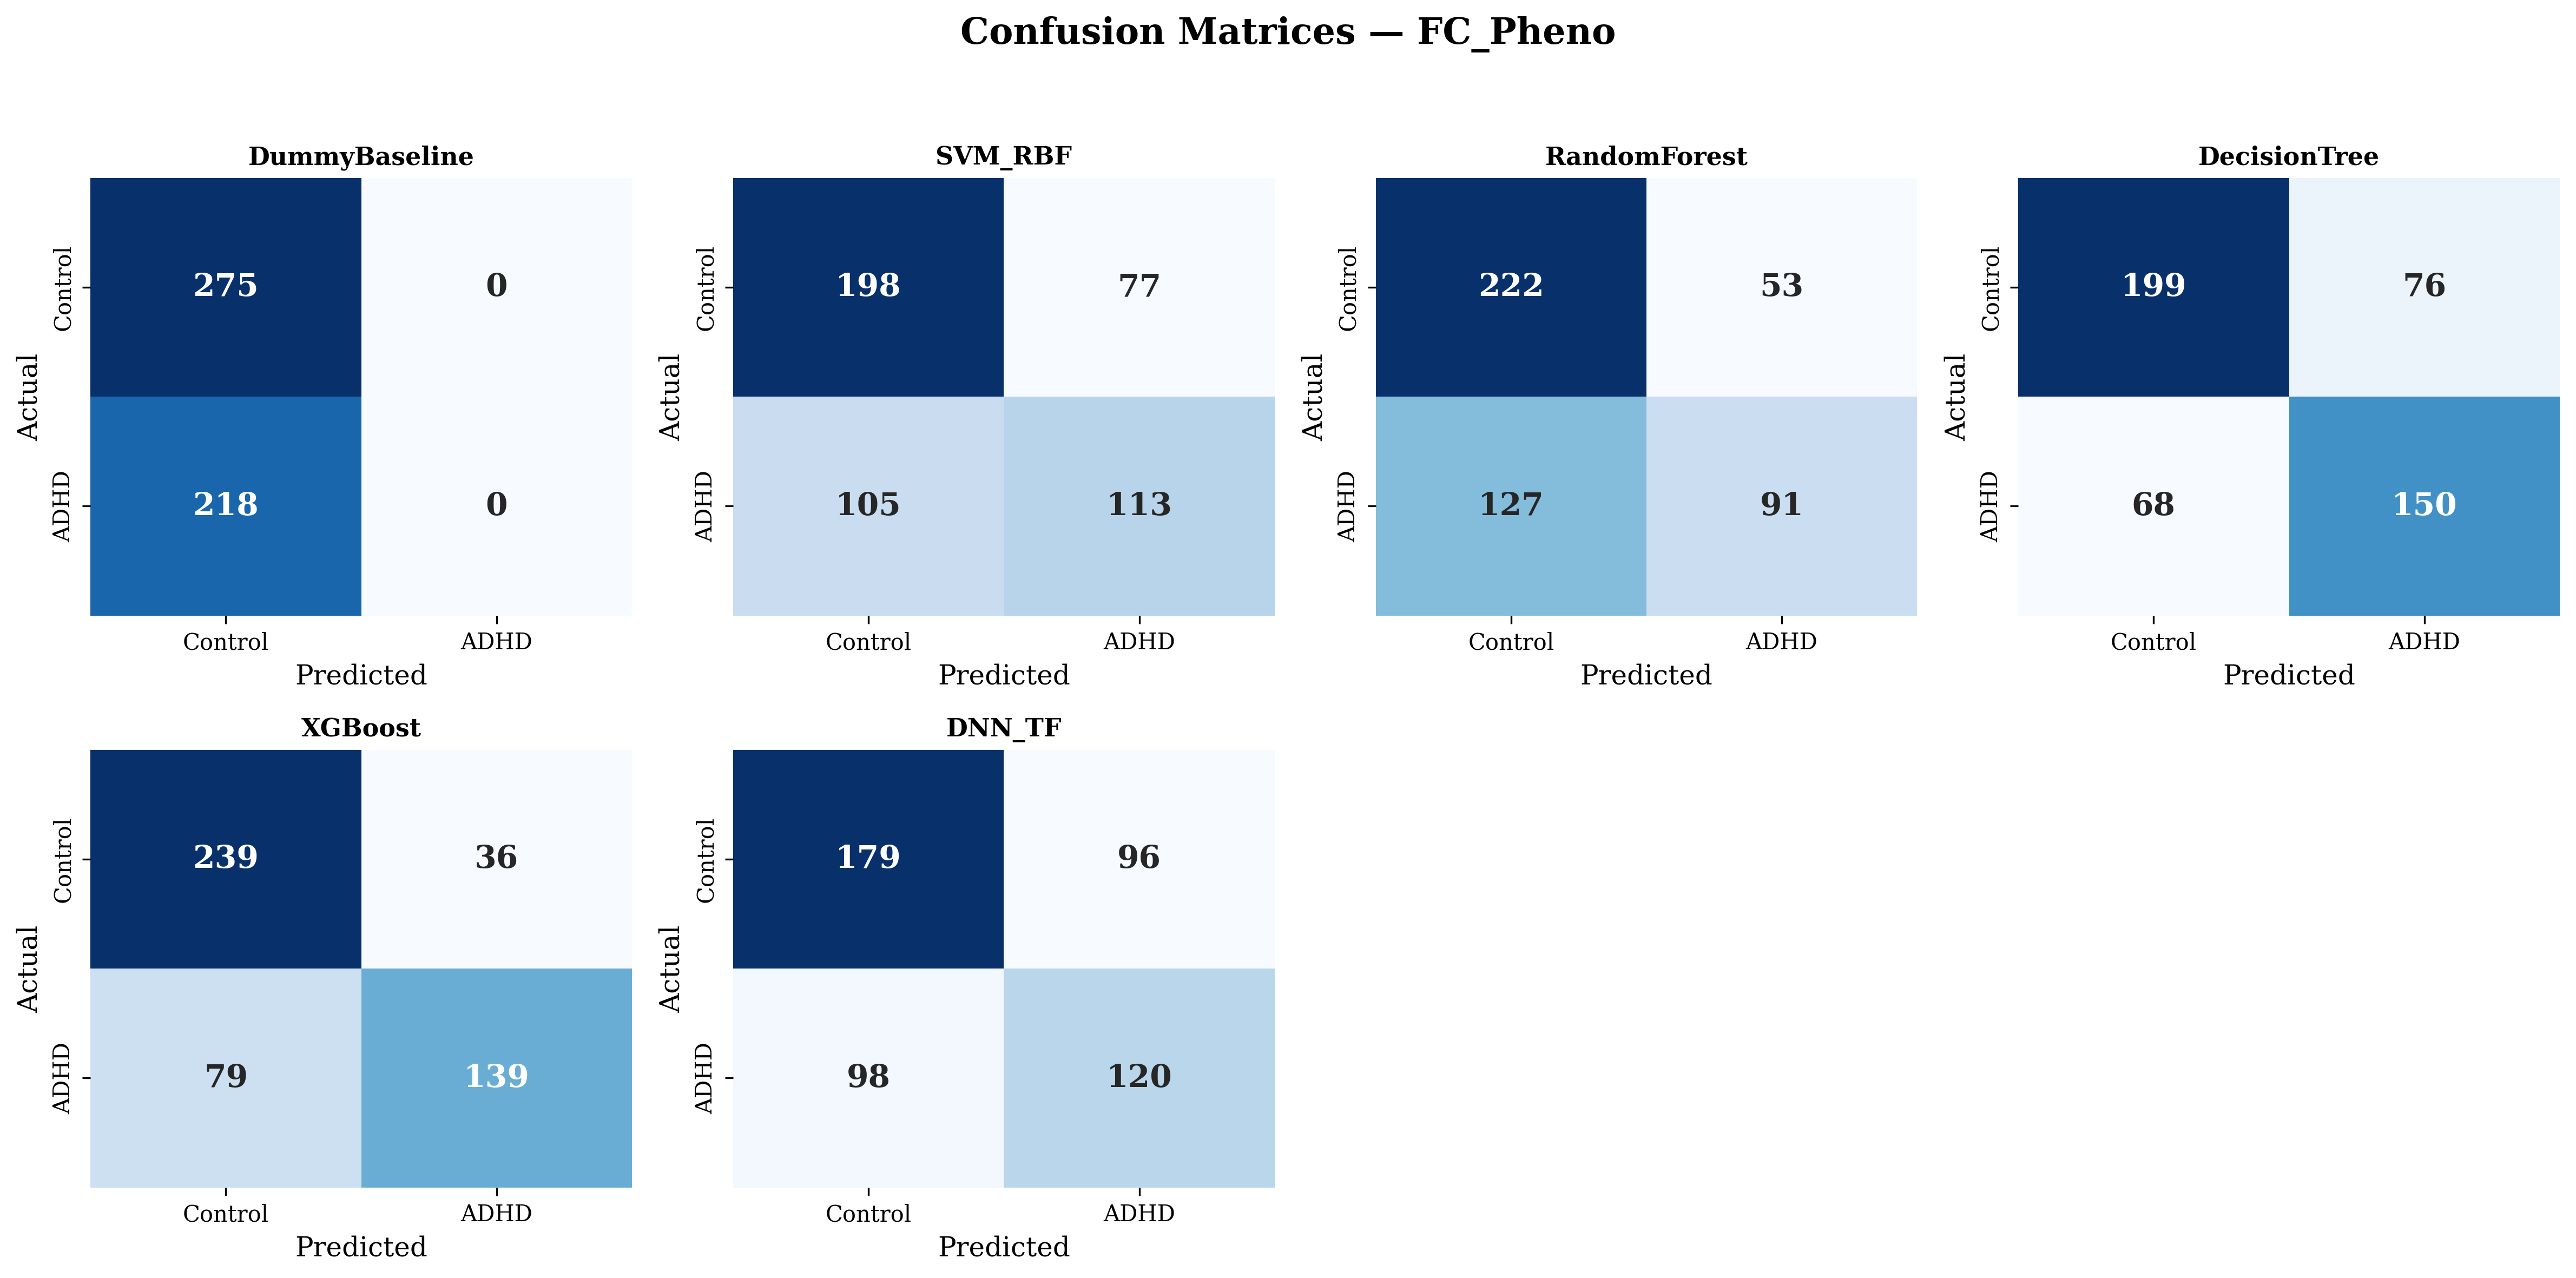
\includegraphics[width=0.62\textwidth]{figures/FC_Pheno_confusion_matrices.png}
\vspace{-3mm}
\caption{Confusion matrices for all models on the FC+Phenotypic feature configuration.}
\label{fig:confusion}
\vspace{-3mm}
\end{figure*}

\subsection{Phenotypic Features}
In addition to imaging-derived features, subject-level phenotypic variables were included to provide demographic and clinical context. The variables retained were: Verbal IQ, Performance IQ, Full4 IQ, Med Status, Age, and Sex. Diagnostic subscale scores (ADHD Index, Inattentive, Hyper/Impulsive) were excluded from the feature set, as these scores are direct clinical measures of the diagnosis itself and their inclusion would constitute data leakage. Numerical features were standardized to zero mean and unit variance. Med Status was binary encoded. For traditional machine learning models, phenotypic features were concatenated with imaging feature vectors to form a unified input.

\begin{figure}[t]
\centering
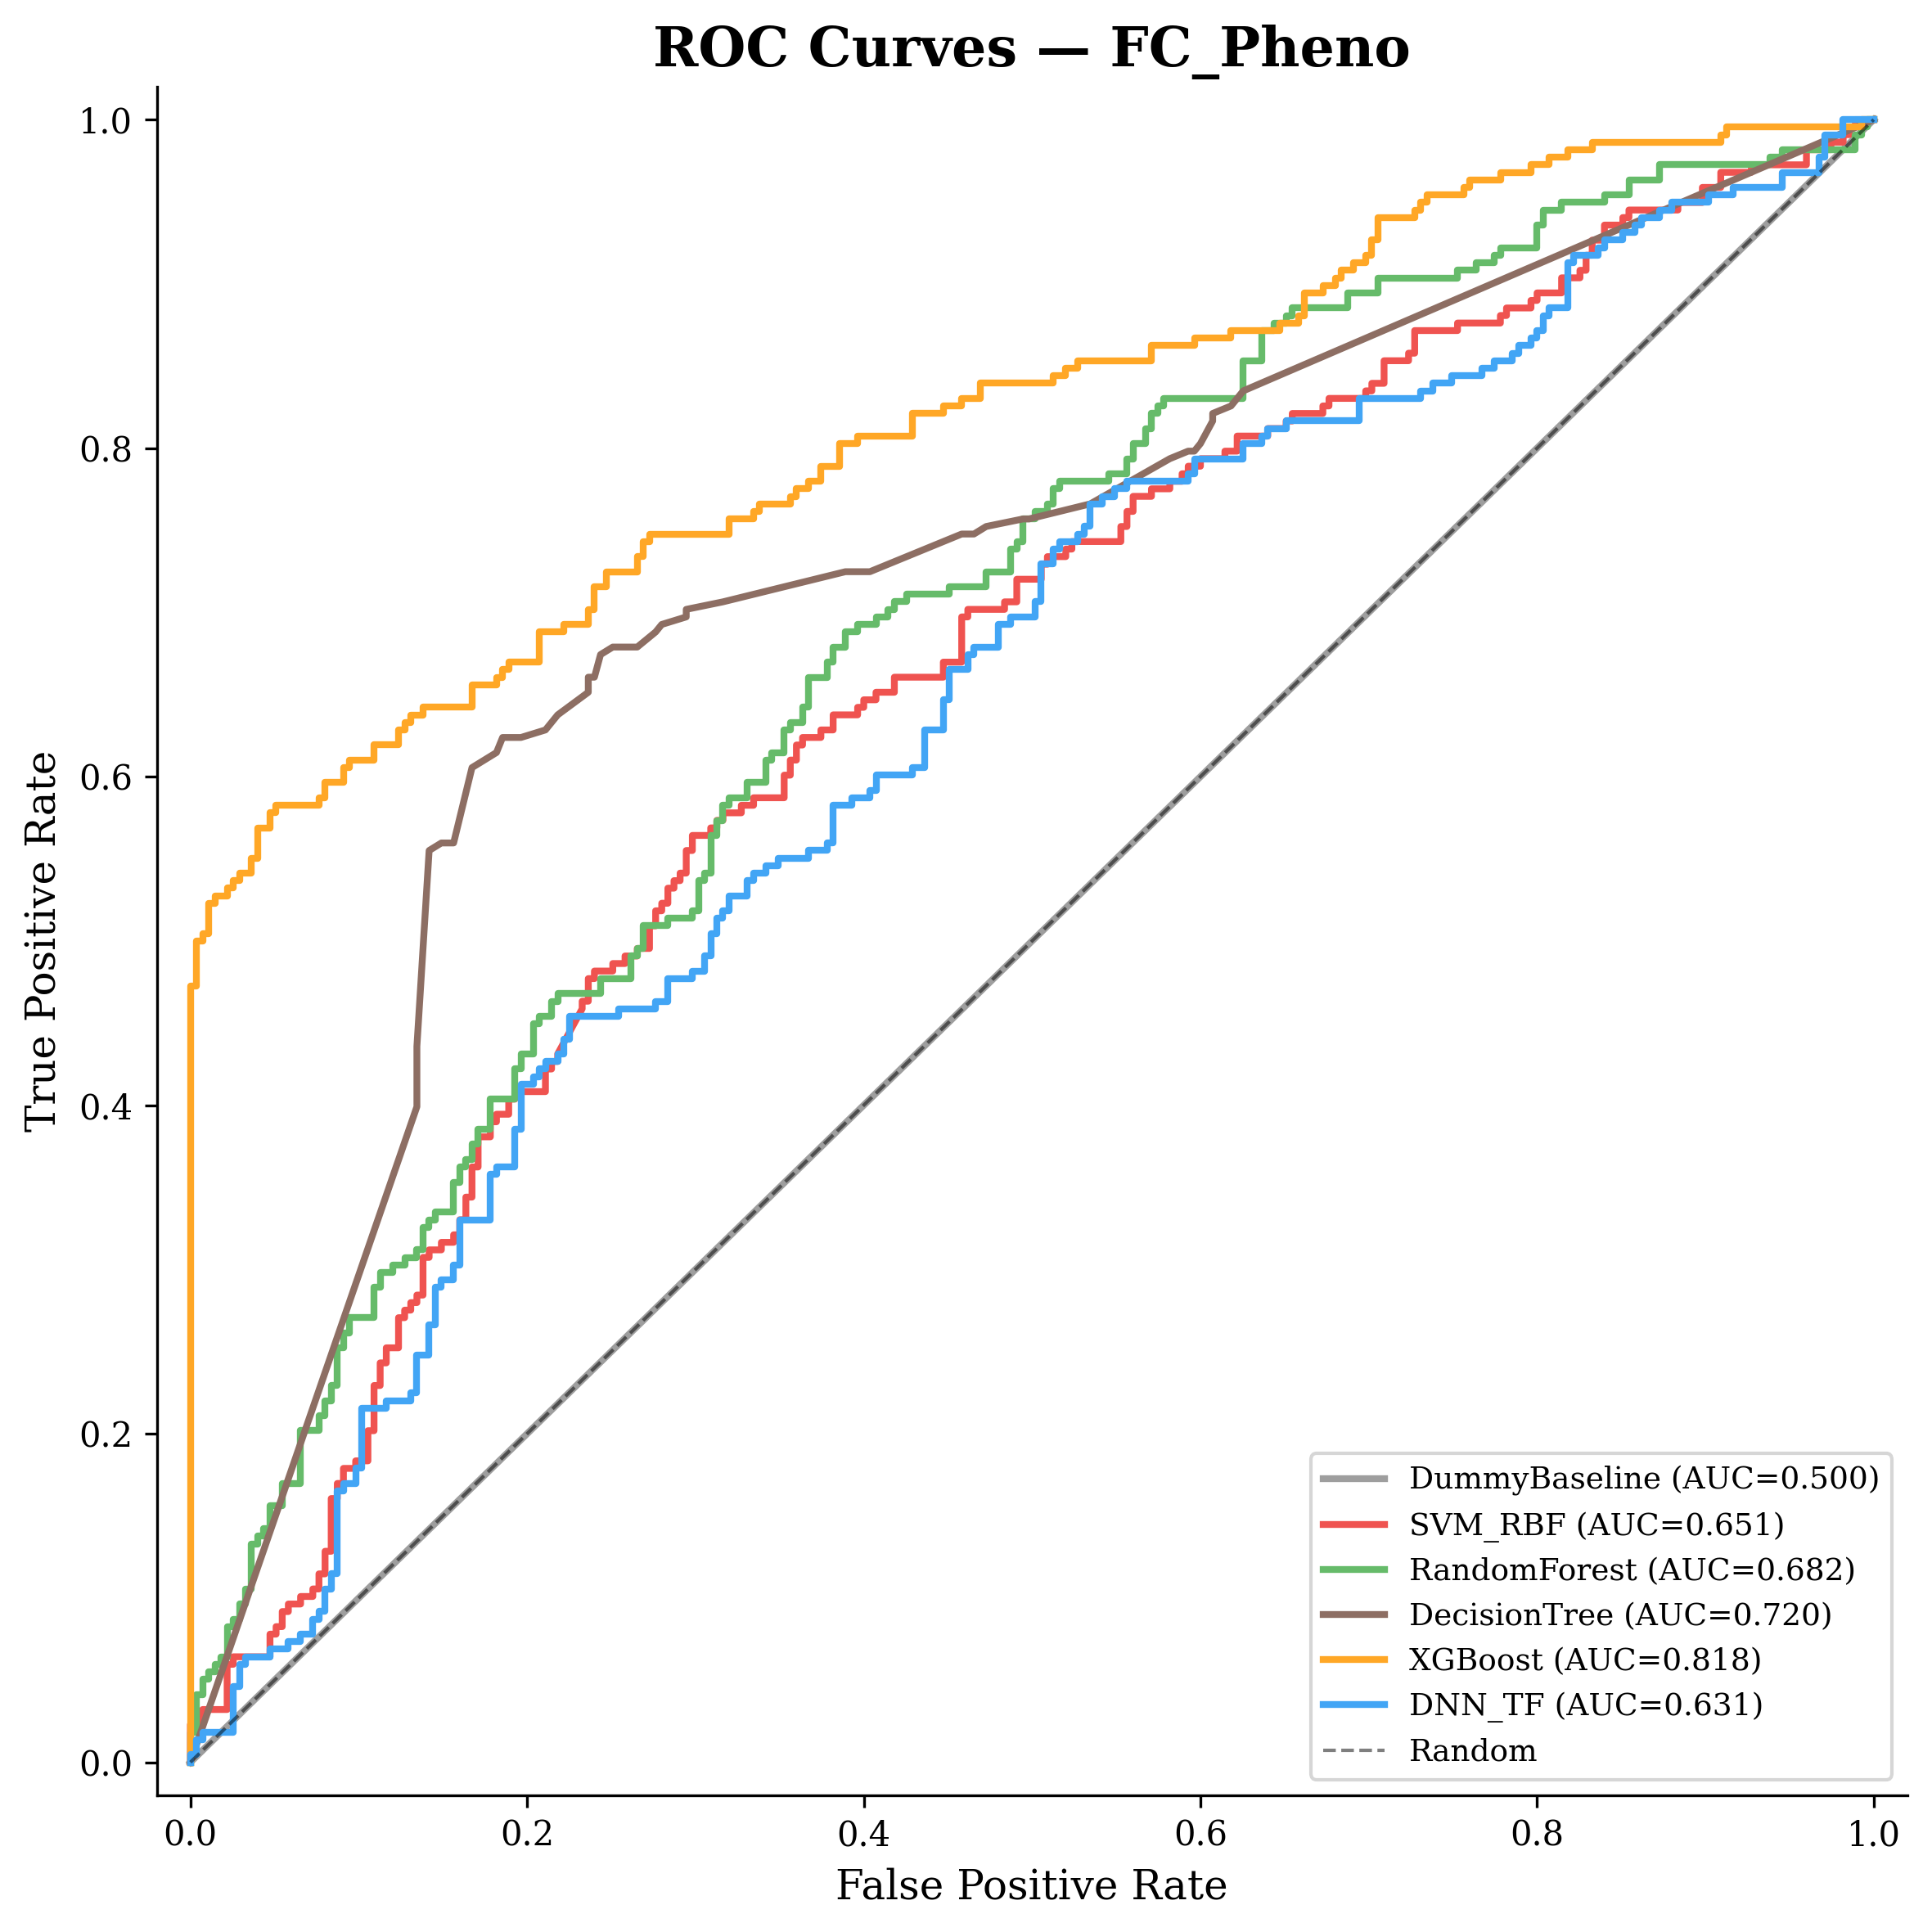
\includegraphics[width=0.60\columnwidth]{figures/FC_Pheno_roc_curves.png}
\vspace{-3mm}
\caption{ROC curves for all models on FC+Pheno. XGBoost achieves the highest AUC of 0.819.}
\label{fig:roc}
\vspace{-3mm}
\end{figure}

\subsection{Machine Learning Models}
This study evaluated five classification models, including both traditional machine learning approaches and a deep learning architecture. All models were trained using combinations of imaging features---functional connectivity (FC), fractional amplitude of low-frequency fluctuations (fALFF), and regional synchrony approximation---and standardized subject-level phenotypic features.

\subsubsection{Traditional Machine Learning Models}
Implementation of four traditional classifiers using scikit-learn and XGBoost: support vector machines (SVMs) with a radial basis function (RBF) kernel, decision trees, random forests, and XGBoost. Each model was trained and evaluated on the 620-subject subset of the ADHD-200 dataset using six structured feature configurations. These included functional connectivity (FC), PCA-reduced FC, fractional amplitude of low-frequency fluctuations (fALFF), and regional synchrony approximation, both independently and in combination, as well as FC combined with phenotypic features.

This evaluation allowed us to assess both algorithmic differences and the value of different feature combinations for ADHD classification. SVMs offered a strong non-linear baseline, while decision trees and random forests provided interpretable classifiers with built-in feature importance metrics. XGBoost, a gradient-boosted ensemble method, consistently achieved the highest classification accuracy across feature configurations, performing particularly well when trained on the combination of imaging and phenotypic features.

\begin{figure*}[t]
\centering
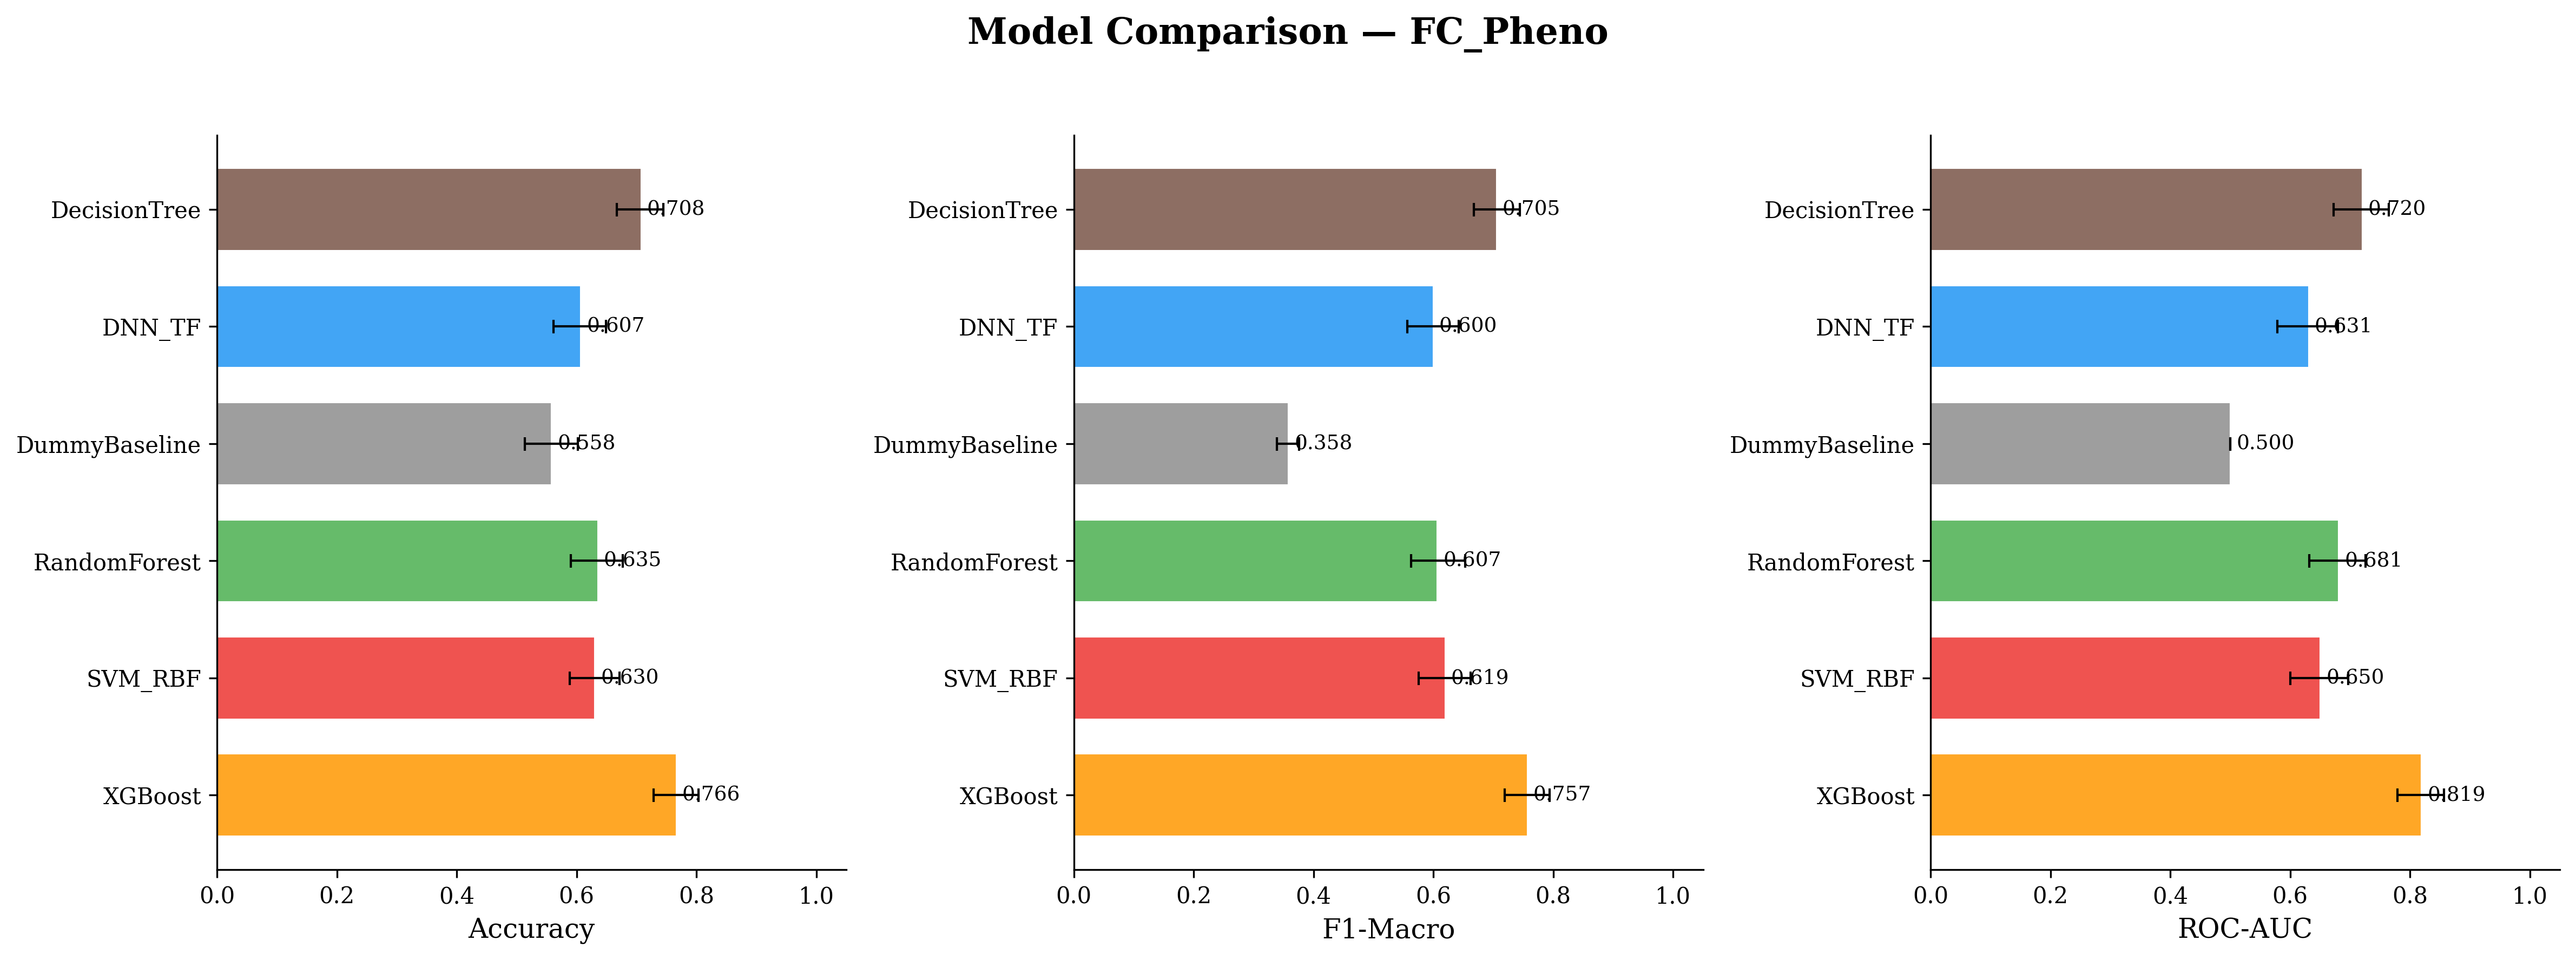
\includegraphics[width=0.60\textwidth]{figures/FC_Pheno_model_comparison.png}
\vspace{-4mm}
\caption{Model comparison on FC+Phenotypic feature configuration showing accuracy, F1-macro, and ROC-AUC metrics with 95\% bootstrap confidence intervals.}
\label{fig:comparison}
\vspace{-4mm}
\end{figure*}

Table~\ref{tab:model_overview} summarizes the models, input features, and architectural characteristics.

\begin{table}[t]
\caption{Model Inputs and Architectural Overview}
\label{tab:model_overview}
\centering
\small
\begin{tabular}{@{}l p{3.2cm} p{2.8cm}@{}}
\toprule
\textbf{Model} & \textbf{Input Features} & \textbf{Architecture} \\
\midrule
SVM (RBF) & FC, fALFF, ROI Sync, Pheno & Kernel-based RBF classifier \\
\midrule
Decision Tree & FC, fALFF, ROI Sync, Pheno & Single tree with Gini split \\
\midrule
Random Forest & FC, fALFF, ROI Sync, Pheno & Ensemble with majority voting \\
\midrule
XGBoost & FC, fALFF, ROI Sync, Pheno & Gradient-boosted tree ensemble \\
\midrule
DNN & FC, fALFF, ROI Sync, Pheno & MLP with batch norm, dropout \\
\bottomrule
\end{tabular}
\end{table}

\subsubsection{Deep Neural Network (DNN)}
The deep learning model was a multi-layer perceptron (MLP) implemented in TensorFlow/Keras. The network received a flattened feature vector as input and processed it through dense layers with batch normalization, ReLU activations, and dropout regularization, concluding in a sigmoid activation for binary classification. Early stopping was applied with a validation loss monitor to prevent overfitting. Class imbalance was addressed during training by adjusting class weights derived from the distribution of diagnostic labels.

\subsection{Training and Evaluation}
All models were trained and evaluated using stratified 10-fold cross-validation across the full dataset, producing out-of-fold predictions for every subject. This approach avoids the variance inherent in single train/test splits and enables subject-level statistical comparisons between models.

For traditional models (SVM, Decision Tree, Random Forest, XGBoost), hyperparameter tuning was conducted using randomized search with 3-fold inner cross-validation \textit{prior to} the main 10-fold evaluation. This two-stage design prevents information leakage from the test folds into hyperparameter selection. Feature scaling (StandardScaler) was applied within each training fold.

For the DNN, the model was retrained from scratch in each fold with early stopping based on validation loss. Class imbalance was addressed during training by adjusting class weights. All deep networks were trained using the Adam optimizer.

Model performance was reported using accuracy, F1-macro score, and ROC-AUC. Statistical evaluation was performed using bootstrap confidence intervals (2000 iterations, 95\% CI) and McNemar's test comparing the best-performing model against all others on each dataset.

\section{Results}

\begin{figure*}[t]
\centering
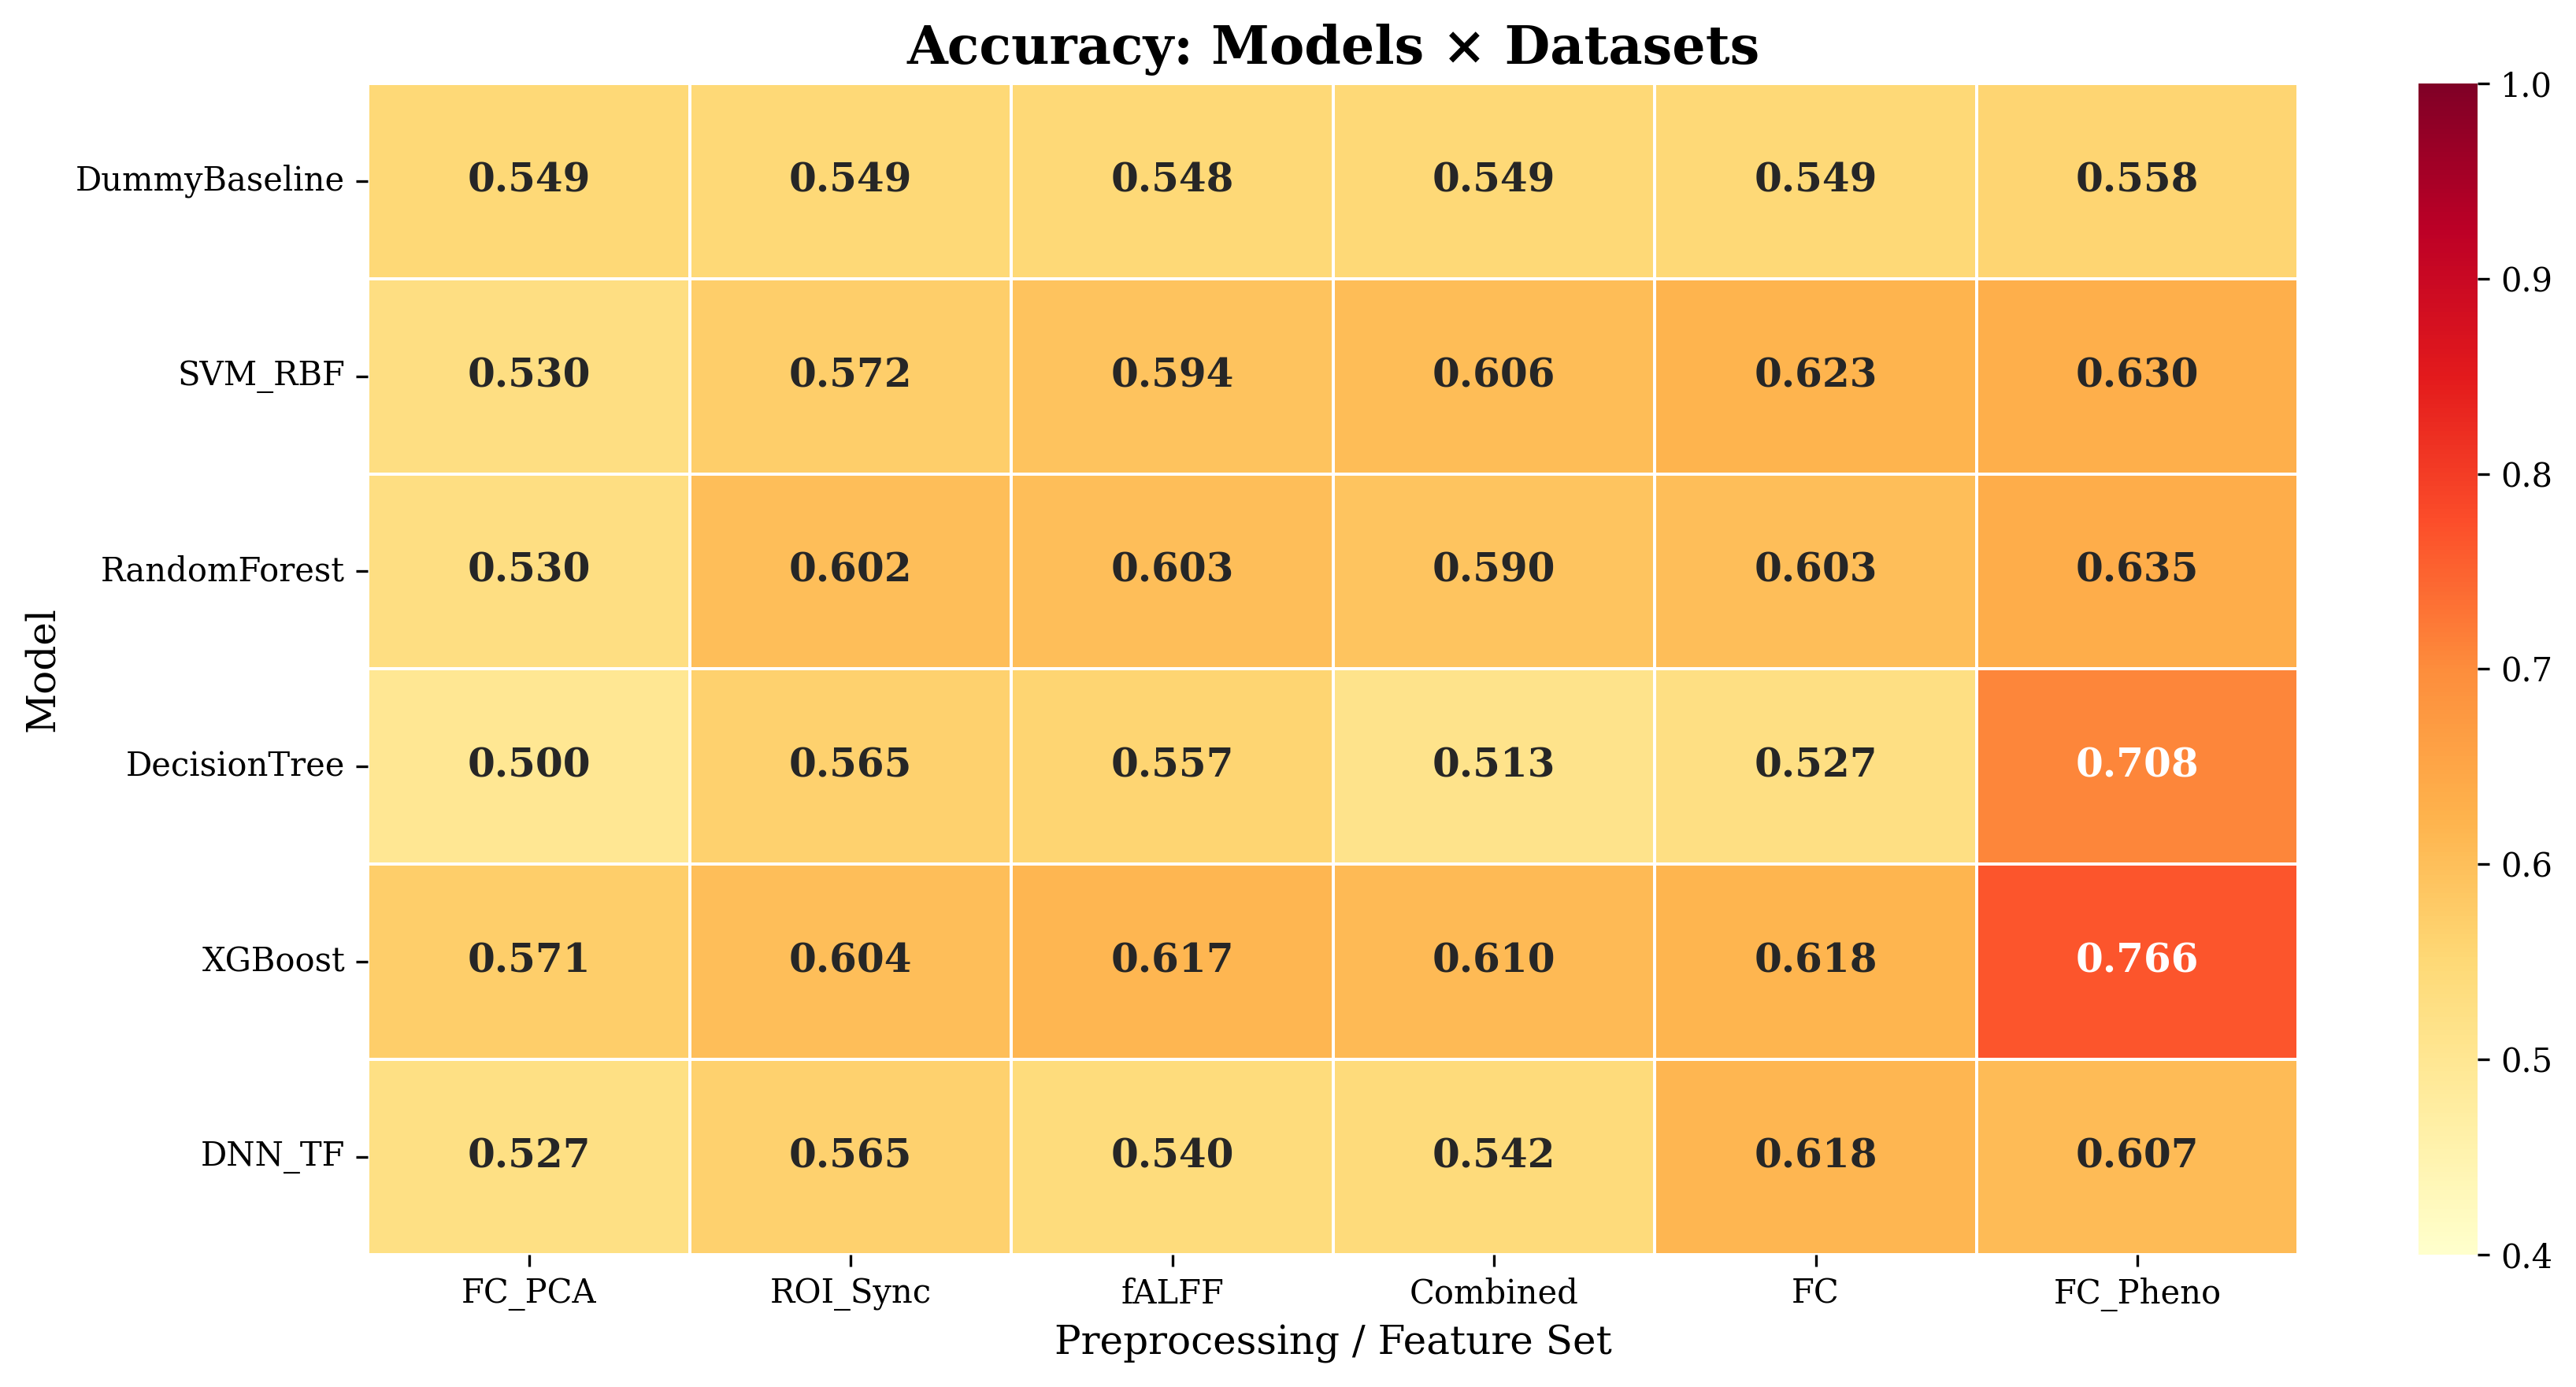
\includegraphics[width=0.48\textwidth]{figures/accuracy_heatmap.png}
\vspace{-4mm}
\caption{Accuracy heatmap across all model--dataset combinations. FC+Pheno (rightmost column) consistently outperforms imaging-only configurations.}
\label{fig:heatmap}
\vspace{-4mm}
\end{figure*}

Table~\ref{tab:results_main} presents the classification performance of all five models on the FC+Phenotypic feature configuration, which produced the highest overall results.

\begin{table}[t]
\caption{Classification Metrics --- FC+Phenotypic Features}
\label{tab:results_main}
\centering
\begin{tabular}{@{}lccc@{}}
\toprule
\textbf{Model} & \textbf{Accuracy} & \textbf{F1-Macro} & \textbf{AUC} \\
\midrule
Dummy Baseline & 55.8\% & 0.358 & 0.500 \\
DNN & 60.7\% & 0.600 & 0.631 \\
SVM (RBF) & 63.0\% & 0.619 & 0.650 \\
Random Forest & 63.5\% & 0.607 & 0.681 \\
Decision Tree & 70.8\% & 0.705 & 0.720 \\
\textbf{XGBoost} & \textbf{76.6\%} & \textbf{0.757} & \textbf{0.819} \\
\bottomrule
\end{tabular}
\end{table}

Among the traditional classifiers, XGBoost achieved the highest overall performance, reaching 76.6\% accuracy and an F1-score of 0.757. Decision Tree also performed well at 70.8\% accuracy, while Random Forest and SVM achieved more modest results around 63\%. These results highlight the strength of gradient-boosted ensemble methods when applied to structured neuroimaging and phenotypic data.

The DNN showed the most modest performance among the trained models at 60.7\% accuracy on FC+Pheno, consistent with findings in the literature that deep learning models require larger datasets to outperform classical methods on structured features.

Table~\ref{tab:results_all} presents accuracy across all 30 model--dataset combinations.

\begin{table}[t]
\caption{Accuracy (\%) Across All Model--Dataset Combinations}
\label{tab:results_all}
\centering
\small
\begin{tabular}{@{}lcccccc@{}}
\toprule
& \textbf{FC\_PCA} & \textbf{ROI\_S} & \textbf{fALFF} & \textbf{Comb} & \textbf{FC} & \textbf{FC\_Ph} \\
\midrule
Dummy & 54.9 & 54.9 & 54.8 & 54.9 & 54.9 & 55.8 \\
DT & 50.0 & 56.5 & 55.7 & 51.3 & 52.7 & 70.8 \\
DNN & 52.7 & 56.5 & 54.0 & 54.2 & 61.8 & 60.7 \\
SVM & 53.0 & 57.2 & 59.4 & 60.6 & 62.3 & 63.0 \\
RF & 53.0 & 60.2 & 60.3 & 59.0 & 60.3 & 63.5 \\
XGB & 57.1 & 60.4 & 61.7 & 61.0 & 61.8 & \textbf{76.6} \\
\bottomrule
\end{tabular}
\end{table}

McNemar's tests confirmed that XGBoost significantly outperformed all other models on FC+Pheno ($p < 0.001$ vs.\ DNN, Random Forest, SVM, and Dummy; $p < 0.01$ vs.\ Decision Tree). On imaging-only datasets, differences between top models were generally not statistically significant.

\section{Discussion}
The results show that ensemble-based traditional models outperformed the deep learning approach in classifying ADHD from rs-fMRI and phenotypic features. This performance gap likely reflects the structured nature of the feature space, which favored tree-based algorithms that excel in handling mixed data types, non-linear interactions, and smaller training sets.

The addition of phenotypic metadata to functional connectivity features produced the largest single improvement in performance across all experiments, with XGBoost accuracy increasing from 61.8\% (FC only) to 76.6\% (FC+Pheno). This underscores that clinical variables such as IQ measures, age, sex, and medication status provide complementary diagnostic information not captured by resting-state brain activity patterns alone.

These findings align with prior studies that have reported robust performance for XGBoost and Random Forest on functional connectivity features \cite{taspinar2024, mahmoud2023}. The imaging-only results (approximately 55--62\% accuracy) are consistent with published benchmarks on the ADHD-200 dataset, where the ADHD-200 Global Competition reported winning accuracies in the 60--67\% range \cite{taspinar2024}.

Several factors contribute to the modest imaging-only performance. ADHD is a heterogeneous disorder with multiple subtypes and varying neurobiological profiles, making it difficult to identify consistent biomarkers across subjects. The multi-site nature of the ADHD-200 dataset introduces variability in scanner hardware, acquisition protocols, and subject demographics. Additionally, PCA-reduced FC features performed notably poorly (50--57\% accuracy), suggesting that aggressive dimensionality reduction discarded discriminative signal.

Several limitations should be considered. The dataset, while larger than many prior studies at 620 subjects, remains modest for training deep learning models. No external validation set was used, and demographic factors such as site effects were not explicitly modeled through domain adaptation. These constraints affect generalizability and highlight the need for broader, more diverse datasets in future work.

Nonetheless, this study contributes a systematic comparison of classical and deep models using multimodal fMRI-derived inputs across multiple feature configurations. The findings suggest that in scenarios where sample size is constrained and input features are structured, traditional machine learning remains a highly competitive option. Future work should explore voxel-level modeling, integrate domain adaptation to account for site differences, investigate sequence-based temporal models such as LSTMs on raw fMRI time series, and evaluate the interpretability of both classical and attention-based models in greater depth.

\section{Conclusion}
This study presented a comprehensive evaluation of traditional machine learning and deep learning models for classifying ADHD using resting-state fMRI and phenotypic features. The results demonstrated that ensemble-based classical classifiers, particularly XGBoost, outperformed the deep learning model when trained on functional connectivity combined with phenotypic features, achieving 76.6\% accuracy and 0.819 AUC. Imaging-only features yielded modest accuracy (55--62\%), consistent with published benchmarks. These findings highlight the effectiveness of combining biologically meaningful fMRI metrics with subject-level metadata and reaffirm the strength of classical models in settings with limited data. Future work should explore voxel-level inputs, domain adaptation across imaging sites, sequence-based temporal modeling, and external validation to further improve model generalizability and clinical relevance.

\section*{Acknowledgment}
This work was supported by Dr.\ Ali Nabi Duman of the University of Houston--Downtown, Department of Mathematics and Statistics, whose guidance and feedback contributed significantly to the development of this research.

\begin{thebibliography}{10}
\small
\setlength{\itemsep}{0pt}
\setlength{\parskip}{0pt}
\bibitem{thomas2015}
R.~Thomas, S.~Sanders, J.~Doust, E.~Beller, and P.~Glasziou, ``Prevalence of attention-deficit/hyperactivity disorder: a systematic review and meta-analysis,'' \textit{Pediatrics}, vol.~135, no.~4, pp.~e994--e1001, Apr.~2015.

\bibitem{zhang2020}
H.~Zhang, Y.~Zhao, W.~Cao, \textit{et al.}, ``Aberrant functional connectivity in resting state networks of ADHD patients revealed by independent component analysis,'' \textit{BMC Neurosci.}, vol.~21, no.~1, p.~39, 2020.

\bibitem{taspinar2024}
G.~S.~Taspinar, M.~Baykara, and I.~Taspinar, ``A review of ADHD detection studies with machine learning methods using rs-fMRI data,'' \textit{NMR Biomed.}, vol.~37, no.~1, p.~e4964, 2024.

\bibitem{leung2016}
D.~W.~M.~Leung \textit{et al.}, ``Functional connectivity-based classification of ADHD using different atlases,'' in \textit{Proc. IEEE EMBS}, 2016, pp.~5981--5984.

\bibitem{mahmoud2023}
S.~M.~Mahmoud and M.~Samy, ``Developing system-based artificial intelligence models for detecting the ADHD,'' \textit{Multimedia Tools and Applications}, vol.~82, pp.~15837--15855, 2023.

\bibitem{zou2017}
L.~Zou \textit{et al.}, ``3D CNN-based automatic diagnosis of Attention Deficit Hyperactivity Disorder using functional and structural MRI,'' \textit{IEEE Access}, vol.~5, pp.~23626--23636, 2017.

\bibitem{mohamed2022}
M.~S.~E.~Mohamed and A.~M.~A.~Ibrahim, ``A short report on ADHD detection using CNN,'' in \textit{Proc. IEEE ICCES}, 2022, pp.~1--4.

\bibitem{kumawat2023}
R.~Kumawat and R.~K.~Dwivedi, ``A class activation map-based interpretable transfer learning model for automated detection of ADHD from fMRI data,'' \textit{Brain Informatics}, vol.~10, no.~1, pp.~1--13, 2023.

\bibitem{elsherif2023}
M.~El-Sherif and D.~El-Kenawy, ``A novel knowledge distillation-based feature selection for the classification of ADHD,'' \textit{Biomed. Signal Process. Control}, vol.~80, p.~104368, 2023.

\bibitem{neurobureau}
The Neuro Bureau, ``The ADHD-200 Preprocessed Repository -- Athena Pipeline,'' [Online]. Available: \url{https://www.nitrc.org/plugins/mwiki/index.php/neurobureau:AthenaPipeline}

\end{thebibliography}

\end{document}
